\documentclass[12pt]{article}
\usepackage[utf8]{inputenc}
\usepackage[T1]{fontenc}
\usepackage[spanish, es-noshorthands,activeacute]{babel}
\usepackage[pdftex,usenames,dvipsnames]{color}
\usepackage{amsmath}
\usepackage{amssymb}
%\usepackage{mathpazo}
%\usepackage{color}
\usepackage{fancyhdr}
\usepackage{graphicx}
\graphicspath{ {./ImgsPr3/} }
\usepackage{wrapfig}
%\usepackage[shortlabels]{enumitem}
%\usepackage{bm}
%\usepackage{lastpage}
%\usepackage{enumitem}
\usepackage{subcaption}
\usepackage{graphicx}
\usepackage{whilecode2}
\DeclareCaptionFormat{custom}
{%
    \textbf{#1#2}\textit{\small #3}
}
\captionsetup{format=custom, labelformat=empty}


\parindent=0mm
\renewcommand*{\baselinestretch}{1.1}
\parskip=5mm
\voffset=-10.4mm
\hoffset=-10.4mm
\oddsidemargin=0mm
\topmargin=0mm
\headheight=4.579965mm
\headsep=3.420035mm
\textwidth=180mm
\textheight=251mm
\marginparsep=0mm
\marginparwidth=0mm
\footskip=8mm
\paperwidth=210mm
\paperheight=297mm

\newcounter{exercise}[section]
\newenvironment{exercise}[2][]{\refstepcounter{exercise}\par\medskip
\noindent \textbf{Exercise~\theexercise.  #2\newline} \rmfamily}{\medskip}

\newenvironment{exercise*}[2][]{\refstepcounter{exercise}\par\medskip
\noindent \textbf{Exercise~\theexercise.  #2\newline} \rmfamily}{\medskip}

\newenvironment{ejercicio}[2][]{\refstepcounter{exercise}\par\medskip
\noindent \textbf{Ejercicio~\theexercise.  #2\newline} \rmfamily}{\medskip}

\newenvironment{apartado}[2][]{\refstepcounter{exercise}\par\medskip
\noindent \textbf{Apartado~\theexercise.  #2\newline} }{\medskip}

\newenvironment{inlinedefinition}[2]
    {\begin{center}
    \begin{tabular}{p{0.9\textwidth}}
    
    \textit{\textbf{#1}.}
    }
    { 
    
    \end{tabular} 
    \end{center}
    }

\pagestyle{fancy}
\fancyhf{}
\lhead{\footnotesize{Teoría de Autómatas y Lenguajes Formales}}
\rhead{\footnotesize{Práctica III}}
\lfoot{\footnotesize{Carlos Martínez Zurita}}
\rfoot{\footnotesize{\thepage}}
\renewcommand{\footrulewidth}{1pt}
\renewcommand{\headrulewidth}{1pt}
\begin{document}
	\begin{apartado}{Describe la máquina de Turing en JFLAP y adjuntar imagen de la misma tras comprobar su funcionamien}
	\begin{figure}[h]
	\centering
	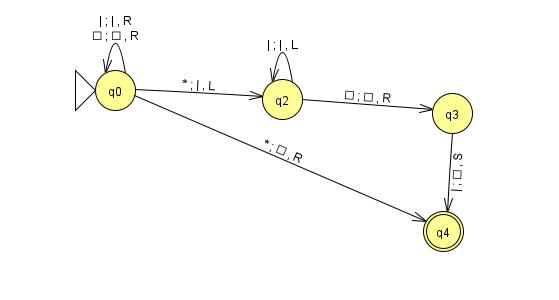
\includegraphics[width=0.4\textwidth]{TMadder}
	\caption{Representación de la máquina de Turing. Funciona incluso cuando una de las cadenas, o ambas, son vacías.}
	\label{fig:figure1}
	\end{figure}
	\end{apartado}
	\begin{apartado}{Describe en Octave una función recursiva que suma tres valores}
	\par{Para definir la funcion recursiva, empezamos pensando en propiedades que debe tener la función $\Sigma_3(x,y,z)=x+y+z$, siendo $Sigma_n$ la función que suma $n$ números naturales: $\Sigma_3(x,y,z)=\Sigma_3(x,y+z,0)=\Sigma_2(x,y+z)$, y esto nos permite definir $\Sigma_3$ mediante recursión primitiva: 
	\begin{equation}
	\Sigma_3(x,y,z)=
		\begin{cases}
			\Sigma_2(x,y) & z=0 \\
		 	\sigma(\pi_4^4(x,y,z-1,\Sigma_3(x,y,z-1))) & z>0 \\
		\end{cases}
	\end{equation}
	Nótese que $\sigma(\pi_4^4(x,y,z,w)=w+1$ es la función sucesor del cuarto argumento. Entonces, $$\Sigma_3=\langle \Sigma_2|\sigma(\pi_4^4) \rangle=\langle\langle \pi_1^1|\sigma(\pi_3^3) \rangle| \sigma(\pi_4^4) \rangle$$
	}
	\par{Se ha descrito el autómata de forma que pueda ser reconocido por \textit{recursiveexpression.m}, que se encuentra en el repositorio de la asignatura. 	Este es el resultado de la ejecución: 
	\begin{figure}[h!]
		\centering
  		\begin{subfigure}[b]{0.55\textwidth}
    			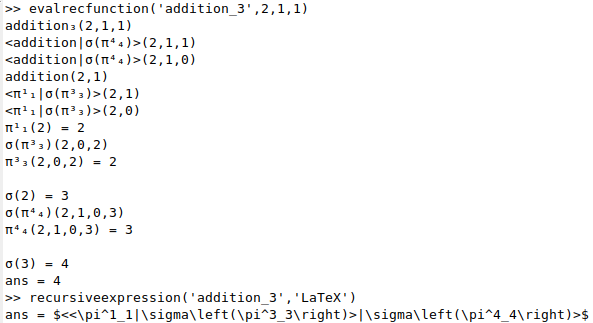
\includegraphics[width=\linewidth]{OctaveSuma3}
  		\end{subfigure}
  		\begin{subfigure}[b]{0.50\textwidth}
    			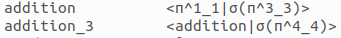
\includegraphics[width=\linewidth]{Suma3Desc}
  		\end{subfigure}
  		\caption{Ejemplo de ejecución de la función recursiva y su definición en Octave}
  		\label{fig:recufuncoctave}
	\end{figure}
	}
	\end{apartado}
	\begin{apartado}{Describe la función que sume tres valores en lenguaje WHILE usando el paquete \texttt{whilecode}}
   		\begin{whilecode}[H]
			\While{$X_3 \not = 0$}{
				$X_4 \Assig X_3 + 1$\;
				$X_3 \Assig X_3 - 1$\;
			}
			\While{$X_2 \not = 0$}{
				$X_4 \Assig X_2 + 1$\;
				$X_2 \Assig X_2 - 1$\;
			}
			\While{$X_1 \not = 0$}{
				$X_4 \Assig X_1 + 1$\;
				$X_1 \Assig X_1 - 1$\;
			}
		\end{whilecode}
	\end{apartado}
\end{document}